\documentclass[10pt, landscape]{article}
\usepackage[scaled=0.92]{helvet}
\usepackage{multicol}
\usepackage{calc}
\usepackage{ifthen}
\usepackage[landscape]{geometry}
%\usepackage{hyperref}

\usepackage{newtxtext} 

%for strikeout
\usepackage{ulem}

%For editing parbox
\usepackage[table]{xcolor}
%For editing itemise margins, reduce iterm separaion and list separation
\usepackage{enumitem}
% For math
\usepackage{amsmath,amsthm,amsfonts,amssymb}

%For pictures / figures
\usepackage{color,graphicx,overpic}
\graphicspath{ {./images/} }

%\usepackage{newtxtext} 
%\usepackage{amssymb}
%\usepackage[table]{xcolor}
%\usepackage{vwcol}
%\usepackage{tikz}
%\usepackage{wrapfig}
%\usepackage{makecell}

\pdfinfo{
  /Title (CS3223-notes.pdf)
  /Creator (Ger Teck)
  /Author (Ger Teck)
  /Subject ()
  /Keywords (tex)}

%% Margins for PAPER

% This sets page margins to .5 inch if using letter paper, and to 1cm
% if using A4 paper. (This probably isn't strictly necessary.)
% If using another size paper, use default 1cm margins.
\ifthenelse{\lengthtest { \paperwidth = 11in}}
	{ \geometry{top=.3in,left=.3in,right=.3in,bottom=.3in} }
	{\ifthenelse{ \lengthtest{ \paperwidth = 297mm}}
		{\geometry{top=0.5cm,left=0.5cm,right=0.5cm,bottom=0.5cm} }
		{\geometry{top=0.5cm,left=0.5cm,right=0.5cm,bottom=0.5cm} }
	}

% Turn off header and footer
\pagestyle{empty}
% for tight centres (less spacing)
\newenvironment{tightcenter}{%
  \setlength\topsep{0.5pt}
  \setlength\parskip{0.5pt}
  \begin{center}
}{%
  \end{center}
}

% Redefine section commands to use less space
\makeatletter
\renewcommand{\section}{\@startsection{section}{1}{0mm}%
                                {-1ex plus -.5ex minus -.2ex}%
                                {0.5ex plus .2ex}%x
                                {\normalfont\large\bfseries}}
\renewcommand{\subsection}{\@startsection{subsection}{2}{0mm}%
                                {-1explus -.5ex minus -.2ex}%
                                {0.5ex plus .2ex}%
                                {\normalfont\normalsize\bfseries}}
\renewcommand{\subsubsection}{\@startsection{subsubsection}{3}{0mm}%
                                {-1ex plus -.5ex minus -.2ex}%
                                {1ex plus .2ex}%
                                {\normalfont\small\bfseries}}
% change font
%\renewcommand{\familydefault}{\sfdefault}
%\renewcommand\rmdefault{\sfdefault}
\linespread{1.05}

\makeatother

% Define BibTeX command
\def\BibTeX{{\rm B\kern-.05em{\sc i\kern-.025em b}\kern-.08em
    T\kern-.1667em\lower.7ex\hbox{E}\kern-.125emX}}

% Don't print section numbers
\setcounter{secnumdepth}{0}

\setlength{\parindent}{0pt}
\setlength{\parskip}{0pt plus 0.5ex}

%% this changes all items (enumerate and itemize, reduce margins) ITEMIZE SEPARATION HERE
\setlength{\leftmargini}{0.5cm}
\setlength{\leftmarginii}{0.5cm}
\setlist[itemize,1]{leftmargin=2mm,labelindent=1mm,labelsep=1mm, itemsep = 0mm}
\setlist[itemize,2]{leftmargin=4mm,labelindent=1mm,labelsep=1mm, itemsep = 0mm}

%itemsep = 0mm
%\setlist{nosep}

% -------------------------------------------------------------------------------

% START OF DOCUMENT HERE

\begin{document}
\raggedright
\footnotesize
\begin{multicols*}{3}

% multicol parameters
% These lengths are set only within the two main columns
%\setlength{\columnseprule}{0.25pt}
\setlength{\premulticols}{1pt}
\setlength{\postmulticols}{1pt}
\setlength{\multicolsep}{1pt}
\setlength{\columnsep}{2pt}

%% DOCUMENT NAME HERE
\begin{center}
     \Large{\textbf{CS3223 Database Sys Implementation}} \\
\end{center}
AY23/24 Sem 2, github.com/gerteck


\section{Introduction}

\subsubsection{Course Details}
\begin{itemize}
\item Prerequisite knowledges: CS2040S, CS2102, CS2106 background (helpful).
\item Reference Textbook: Raghu \& Johannes Database M. Systems, 2002. \\
Encouraged to read ahead based on schedule before the lecture.
\item Course covers data structures, algorithms, different components making up database systems.
\end{itemize}

\centerline{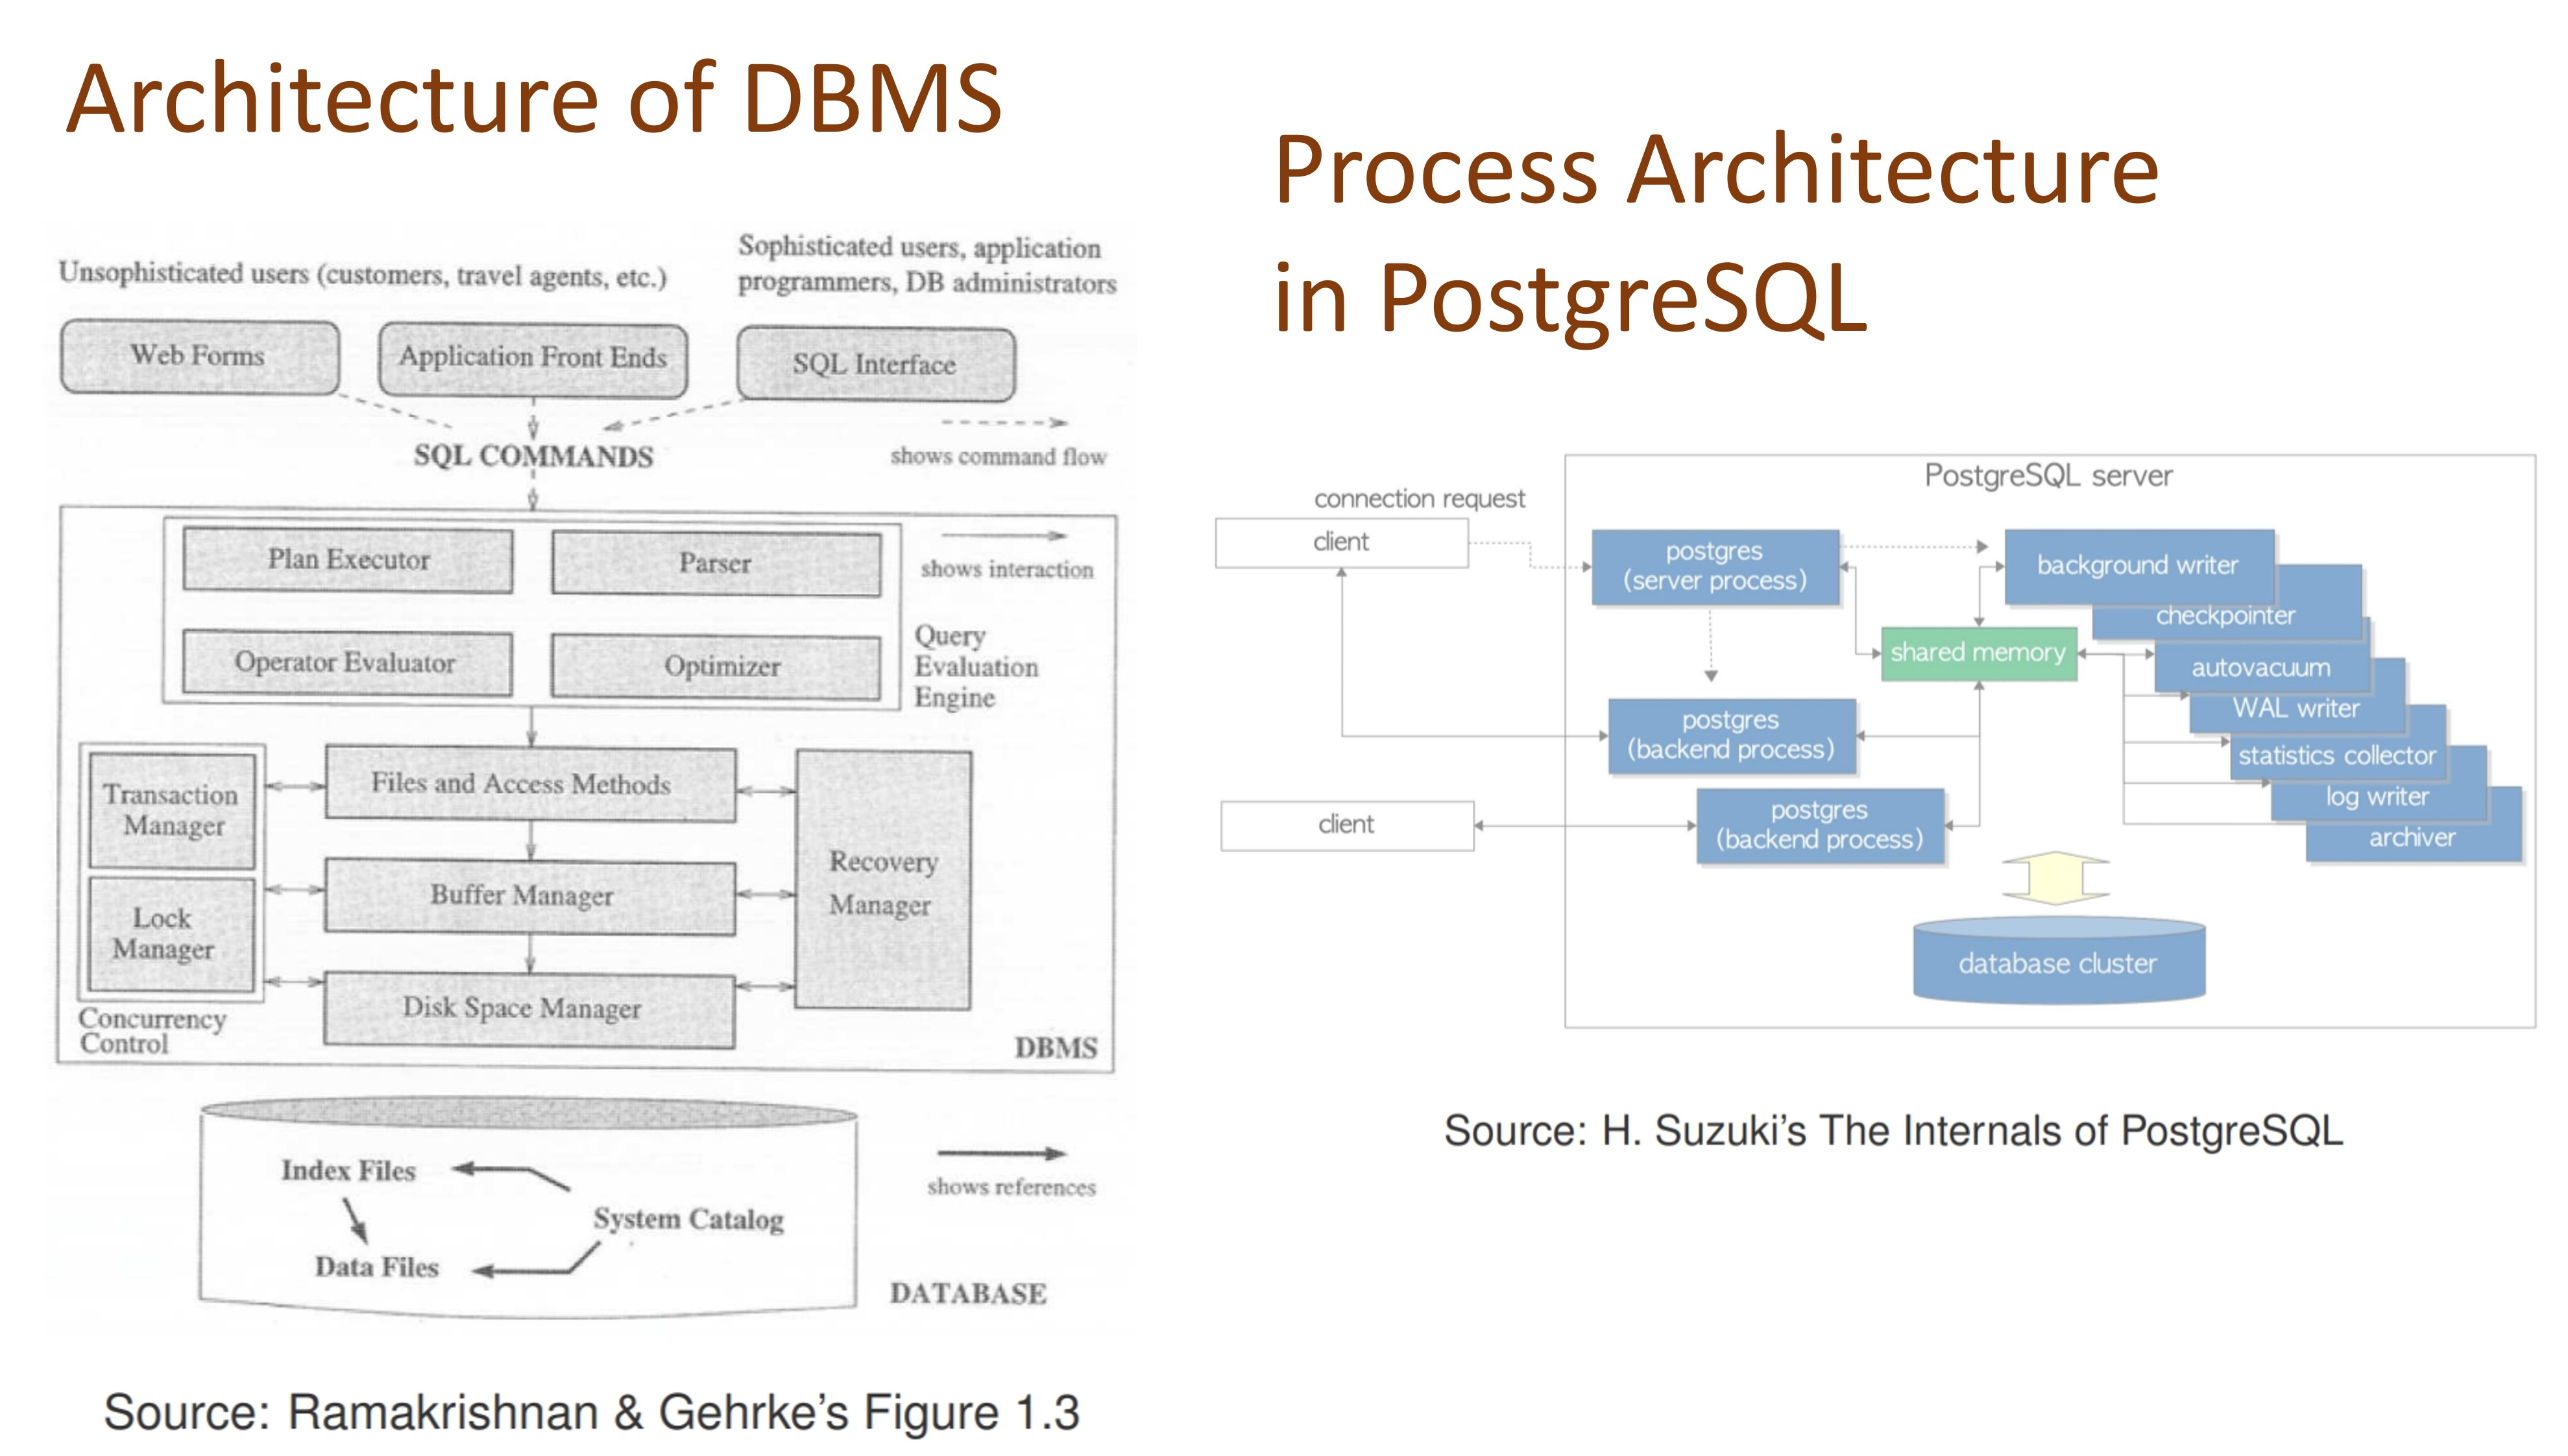
\includegraphics[width = \linewidth]{DBMSArchitecture}}

\begin{itemize}
\item OLTP: Online Transaction Processing is a type of data processing that consists of executing a number of transactions occurring concurrently—online banking, shopping, order entry, or sending text messages, for example.
\item OLAP: Online Analytical Processing.
\item Focusing on centralized database running on a single server.
\end{itemize}

\section{1. Data Storage}
\textbf{References}: R\&G Chapt 8. (Storage \& Indexing Overview), Chapt 9. (Storing Data: Disks and Files).

\subsubsection{A DBMS stores}
\begin{itemize}
\item Relations (Actual tables)
\item System catalog (aka data dictionary) storing metadata about relations.  \\
(Relation schemas, structure of relations, constraints, triggers. View definitions, Indexes - derived info to speed up access to relations, Statistical information about relations for use by query optimizer.) 
\item Log files: Information maintained for data recovery.
\end{itemize}

\subsubsection{DBMS Storage}
\textbf{Memory Hierarchy}: Primary (registers, RAM), secondary (HDD, SSD), tertiary memory with capacity / cost / access speed / volatility tradeoffs.
\begin{itemize}
\item DBMS stores data on non-volatile disk for persistence.
\item DBMS processes data in main memory (RAM).
\item Disk access operations (I/O). Read: transfer data from disk to RAM. Write: transfer data from RAM to disk.
\item Make use of index to speed up access, so that don't have to retrieve all the data when you run a query. Retrieve index and read only the block that contains specified data. Minimize I/O cost.
\end{itemize}

\subsubsection{Magnetic Hard-Disk Drive HDD}
\centerline{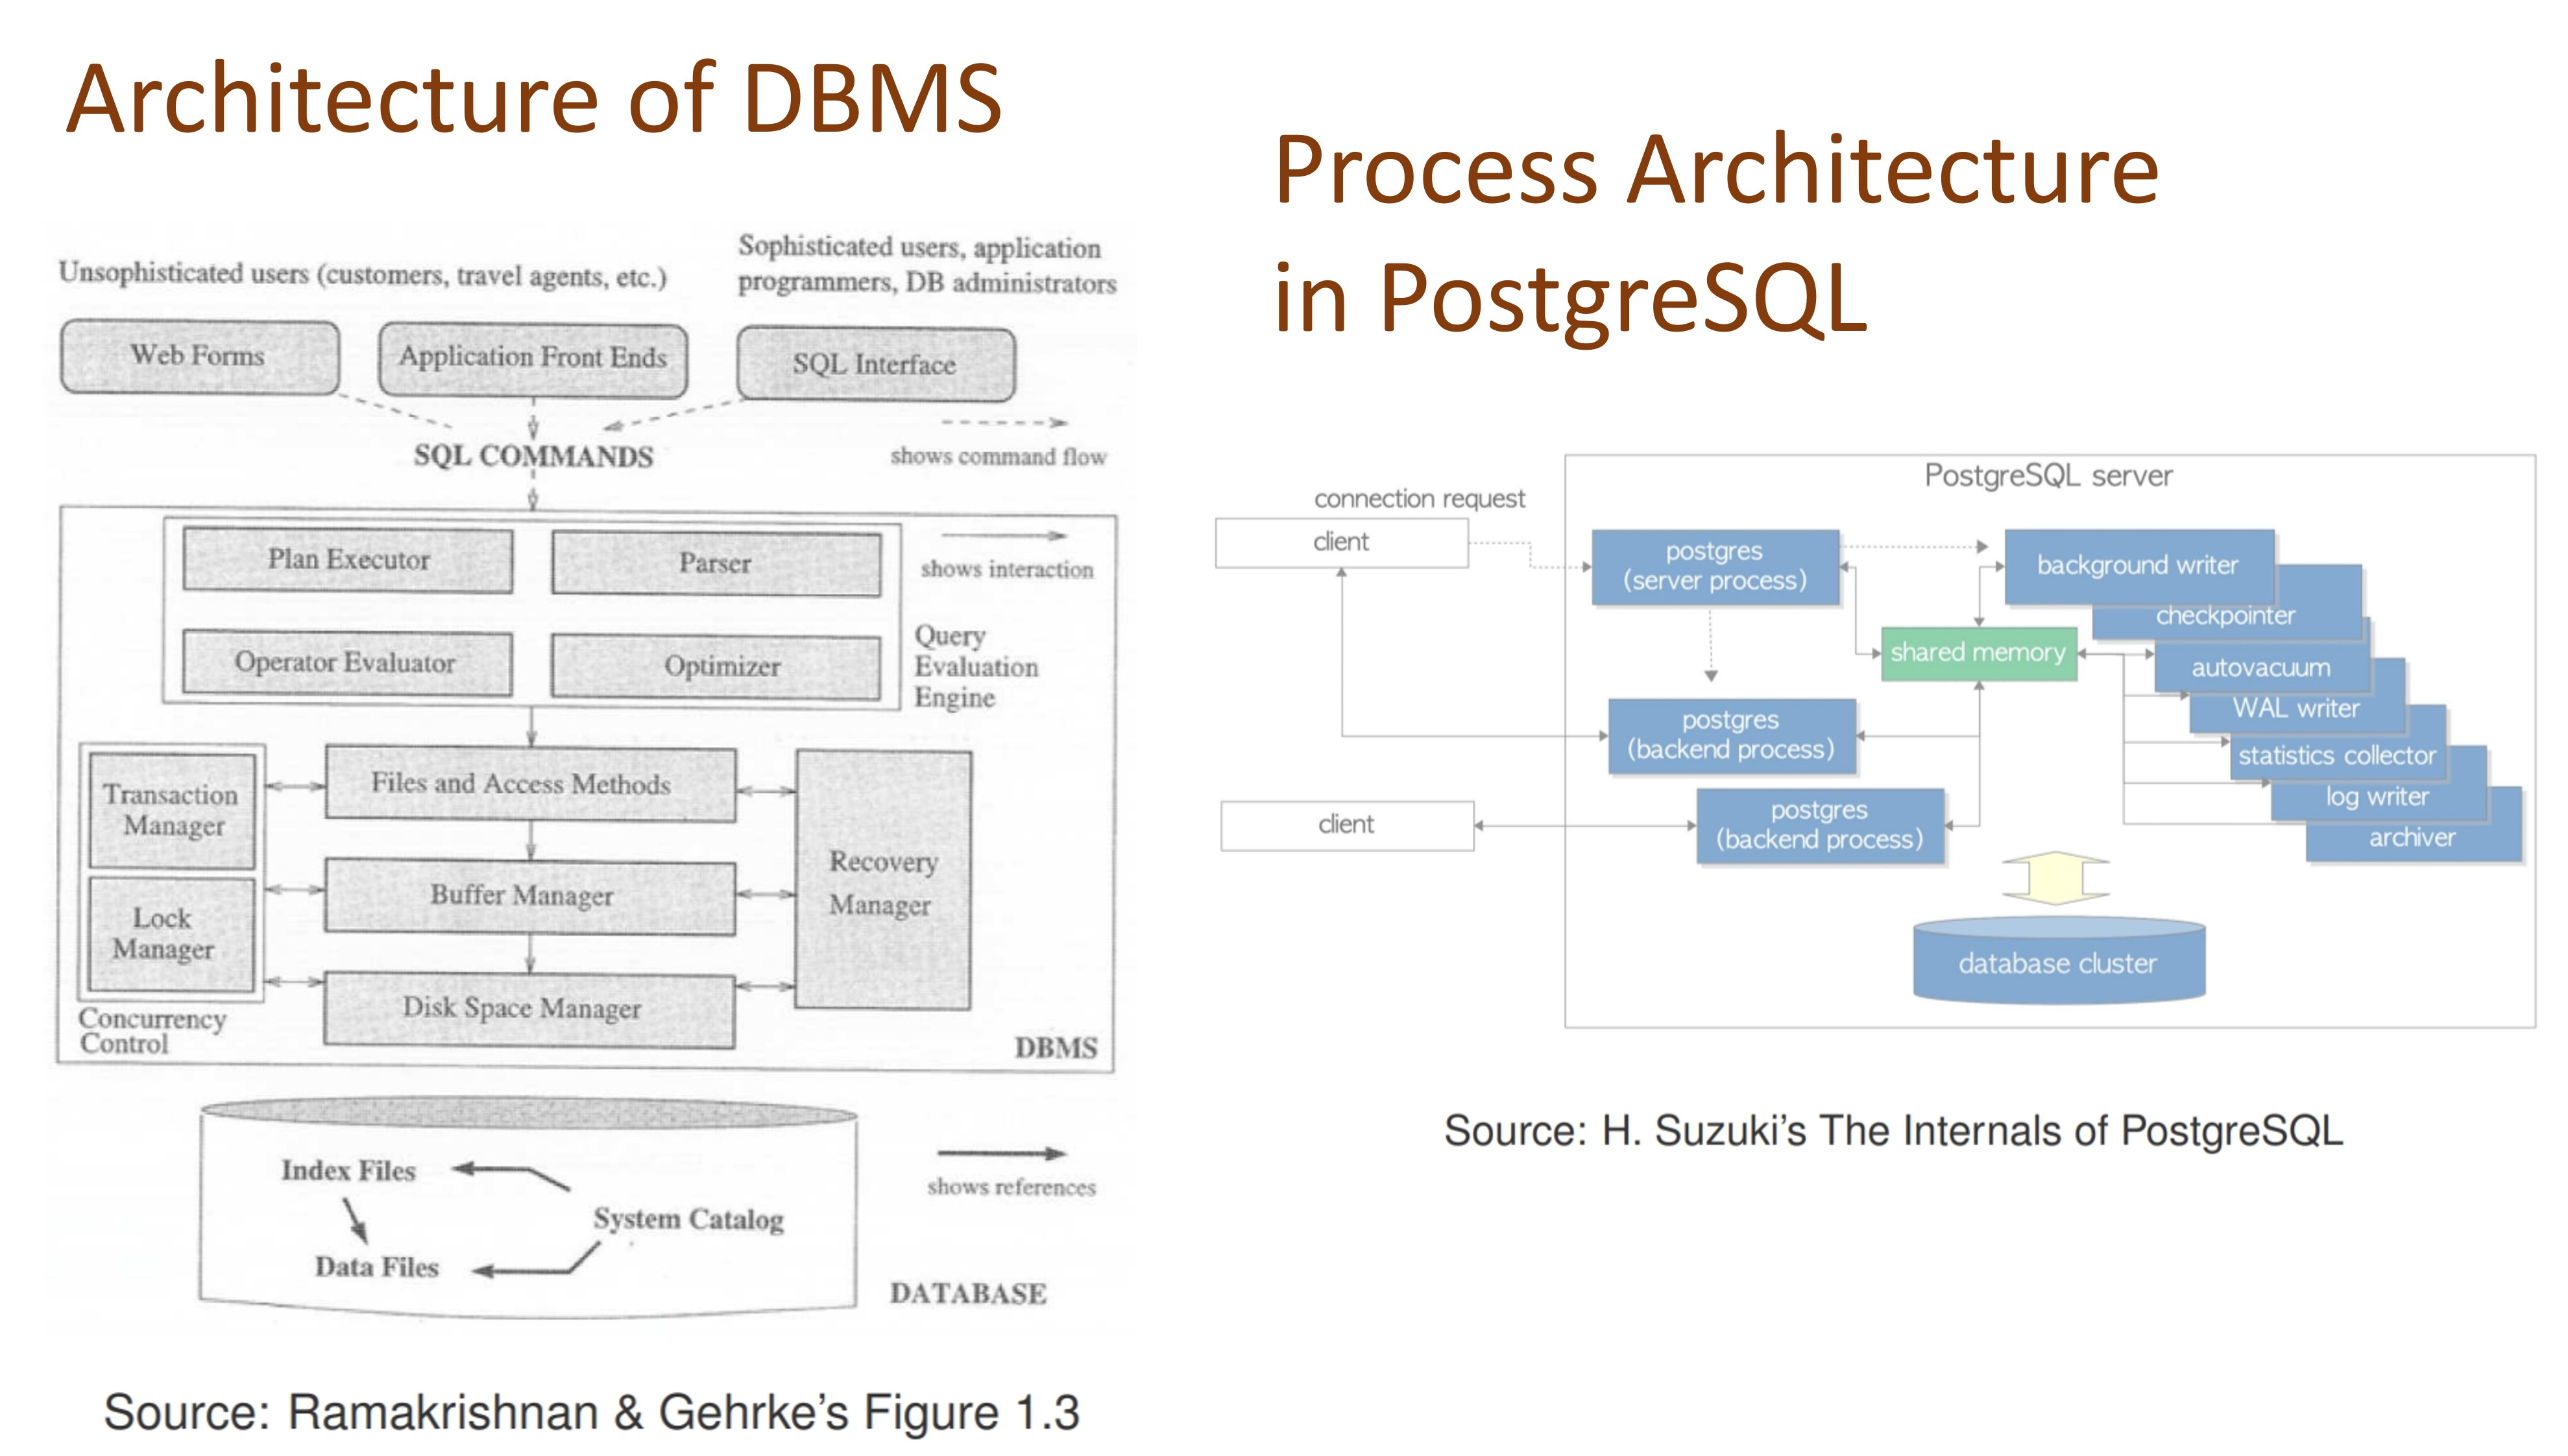
\includegraphics[width = 0.7\linewidth]{DBMSArchitecture}}
\begin{itemize}
\item Cylinder, Track, Sector: Units of the HDD storage system. To read from different tracks, need to move the mechanical HDD arm.
\item \textbf{Disk Access Time}:
	\begin{itemize}
		\item command processing time: interpreting access command by disk controller.
		\item seek time: moving arms to position disk head on track.
		\item rotational delay: waiting for block to rotate under head.
		\item transfer time: actually moving data to/from disk surface.
		\item \textbf{access time}: = seek time + rotational delay + transfer time. (CPT considered negligible). 
	\end{itemize}
\centerline{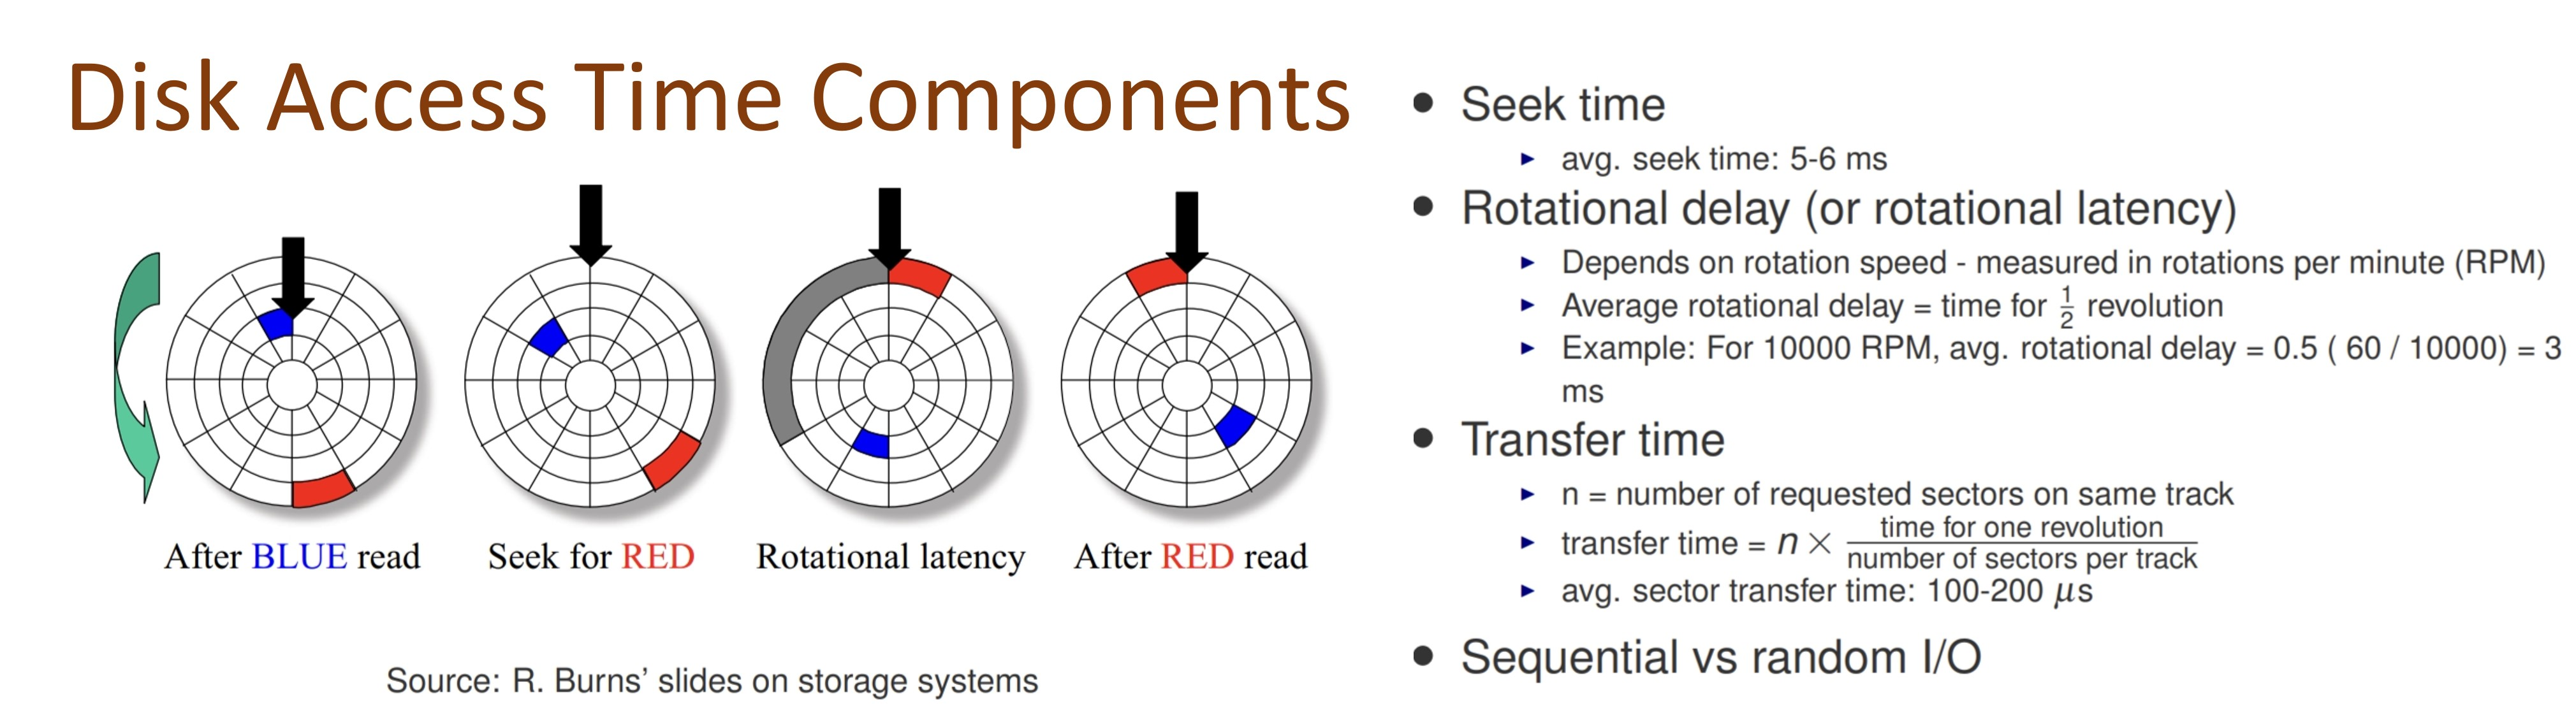
\includegraphics[width = 1\linewidth]{diskAccessTime}}
\item \textbf{Concept of Sequential vs random I/O.} Sequential: Both sector on same track. Random: Sectors on different track, require seeking (moving arm).
\item Given a set of data, we hope to store the data contiguously, on the same track. (Minimize incurring random I/O). If data is too large, store on same track, but different surface (aka same cylinder).
\item Complexity hidden to OS by disk controller. Shown as a sequence of memory locations.
\end{itemize}

\subsubsection{Solid-State Drive: SSD}
\begin{itemize}
\item Build with NAND flash memory without any mechanical moving parts. Lower power consumption.
\item \textbf{Random I/O}: 100x faster than HDD. (no moving parts)
\item \textbf{Sequential I/O}: slightly faster than HDD (~ 2x)
\item \textbf{Disadvantages}: update to a page requires erasure of multiple pages (~ 5ms) before ovewriting page. Limited number of times a page can be erased (~ $10^{5} - 10^{6}$)
\end{itemize}

\subsubsection{Storage Manager Components}
\begin{itemize}
\item Data is stored, retrieved in units called \textbf{disk blocks (or pages}. (Each block = sequence of one or more contiguous sectors.
\item \textbf{FIles \& access methods layer (aka file layer)} - deals with organization and retrieval of data.
\item \textbf{Buffer Manager} - controls reading/writing of disk pages.
\item \textbf{Disk Space Manager} - keeps track of pages used by file layer.
\end{itemize}
\centerline{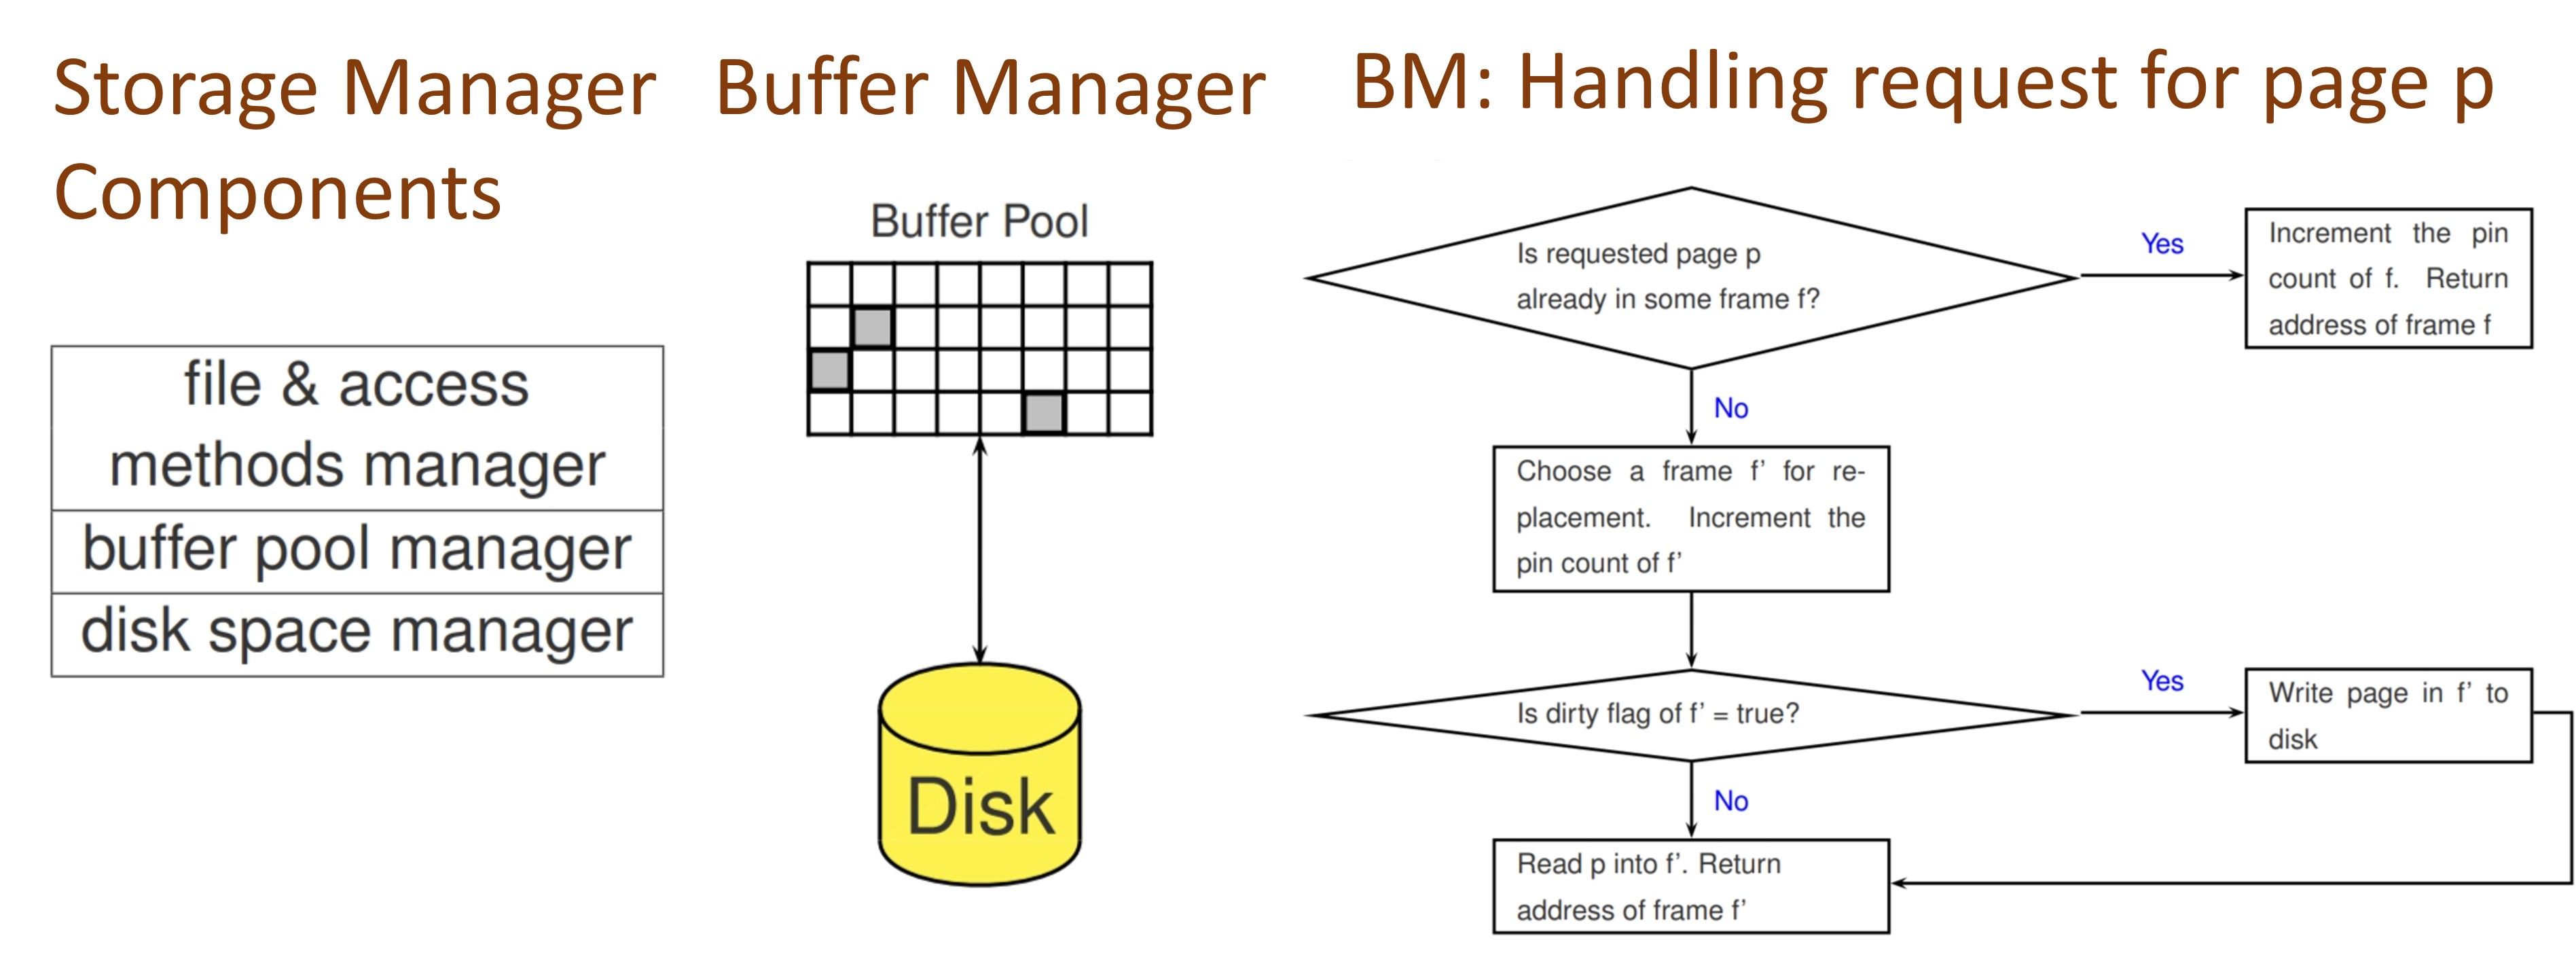
\includegraphics[width = 1\linewidth]{bufferManager}}


\textbf{Buffer Manager}
\begin{itemize}
\item \textbf{Buffer pool}: Main memory allocated for DBMS.
\item Buffer pool is partitioned into block-sized pages called \textbf{frames}.
\item Clients of buffer pool can request for disk page to be fetched into buffer pool, release a disk page in buffer pool.
\item A page in the buffer is \textbf{dirty} if it has been modified \& not updated on disk.
\item \textbf{Two variables} maintained for each frame in buffer pool: 
	\begin{itemize}
		\item \textbf{pin count}: number of clients using page (initialized 0)
		\item \textbf{dirty flag}: whether page is dirty (initialized false)
	\end{itemize}
\item Free list: Keeps track of frames that are free / empty.
\item \textbf{Pin count}: Incrementing pin count is \textbf{pinning} the requested page in its frame. Decrementing is \textbf{unpinning} the page. 
	\begin{itemize}
		\item Unpinning a page, dirty flag should be updated to true if page is dirty.
		\item A page in buffer can be replaced only when pin count is 0. 
		\item Before replacing buffer page, needs to be written back to disk if its dirty flag is true. 
	\end{itemize}
\item Buffer manager coordinates with transaction manager to ensure data correctness and recoverability.
\item \textbf{Replacement Policies}
	\begin{itemize}
		\item Replacement policy: Deciding which unpinned page to replace. (some examples:)
		\item Random, FIFO, Most Recently Used (MRU), Least Recently Used (LRU): (Use queue of pointers to frames with pin count = 0), most common, makes use of temporal locality.
		\item \textbf{Clock}: cheaper popular variant of LRU \\
		- \textbf{current} variable: points to some buffer frame. \\
		- Each frame has a \textbf{referenced bit}, turns on when its pin count turns 0. \\
		- Replace a page that has referenced bit off \& pin count = 0.
	\end{itemize}
\centerline{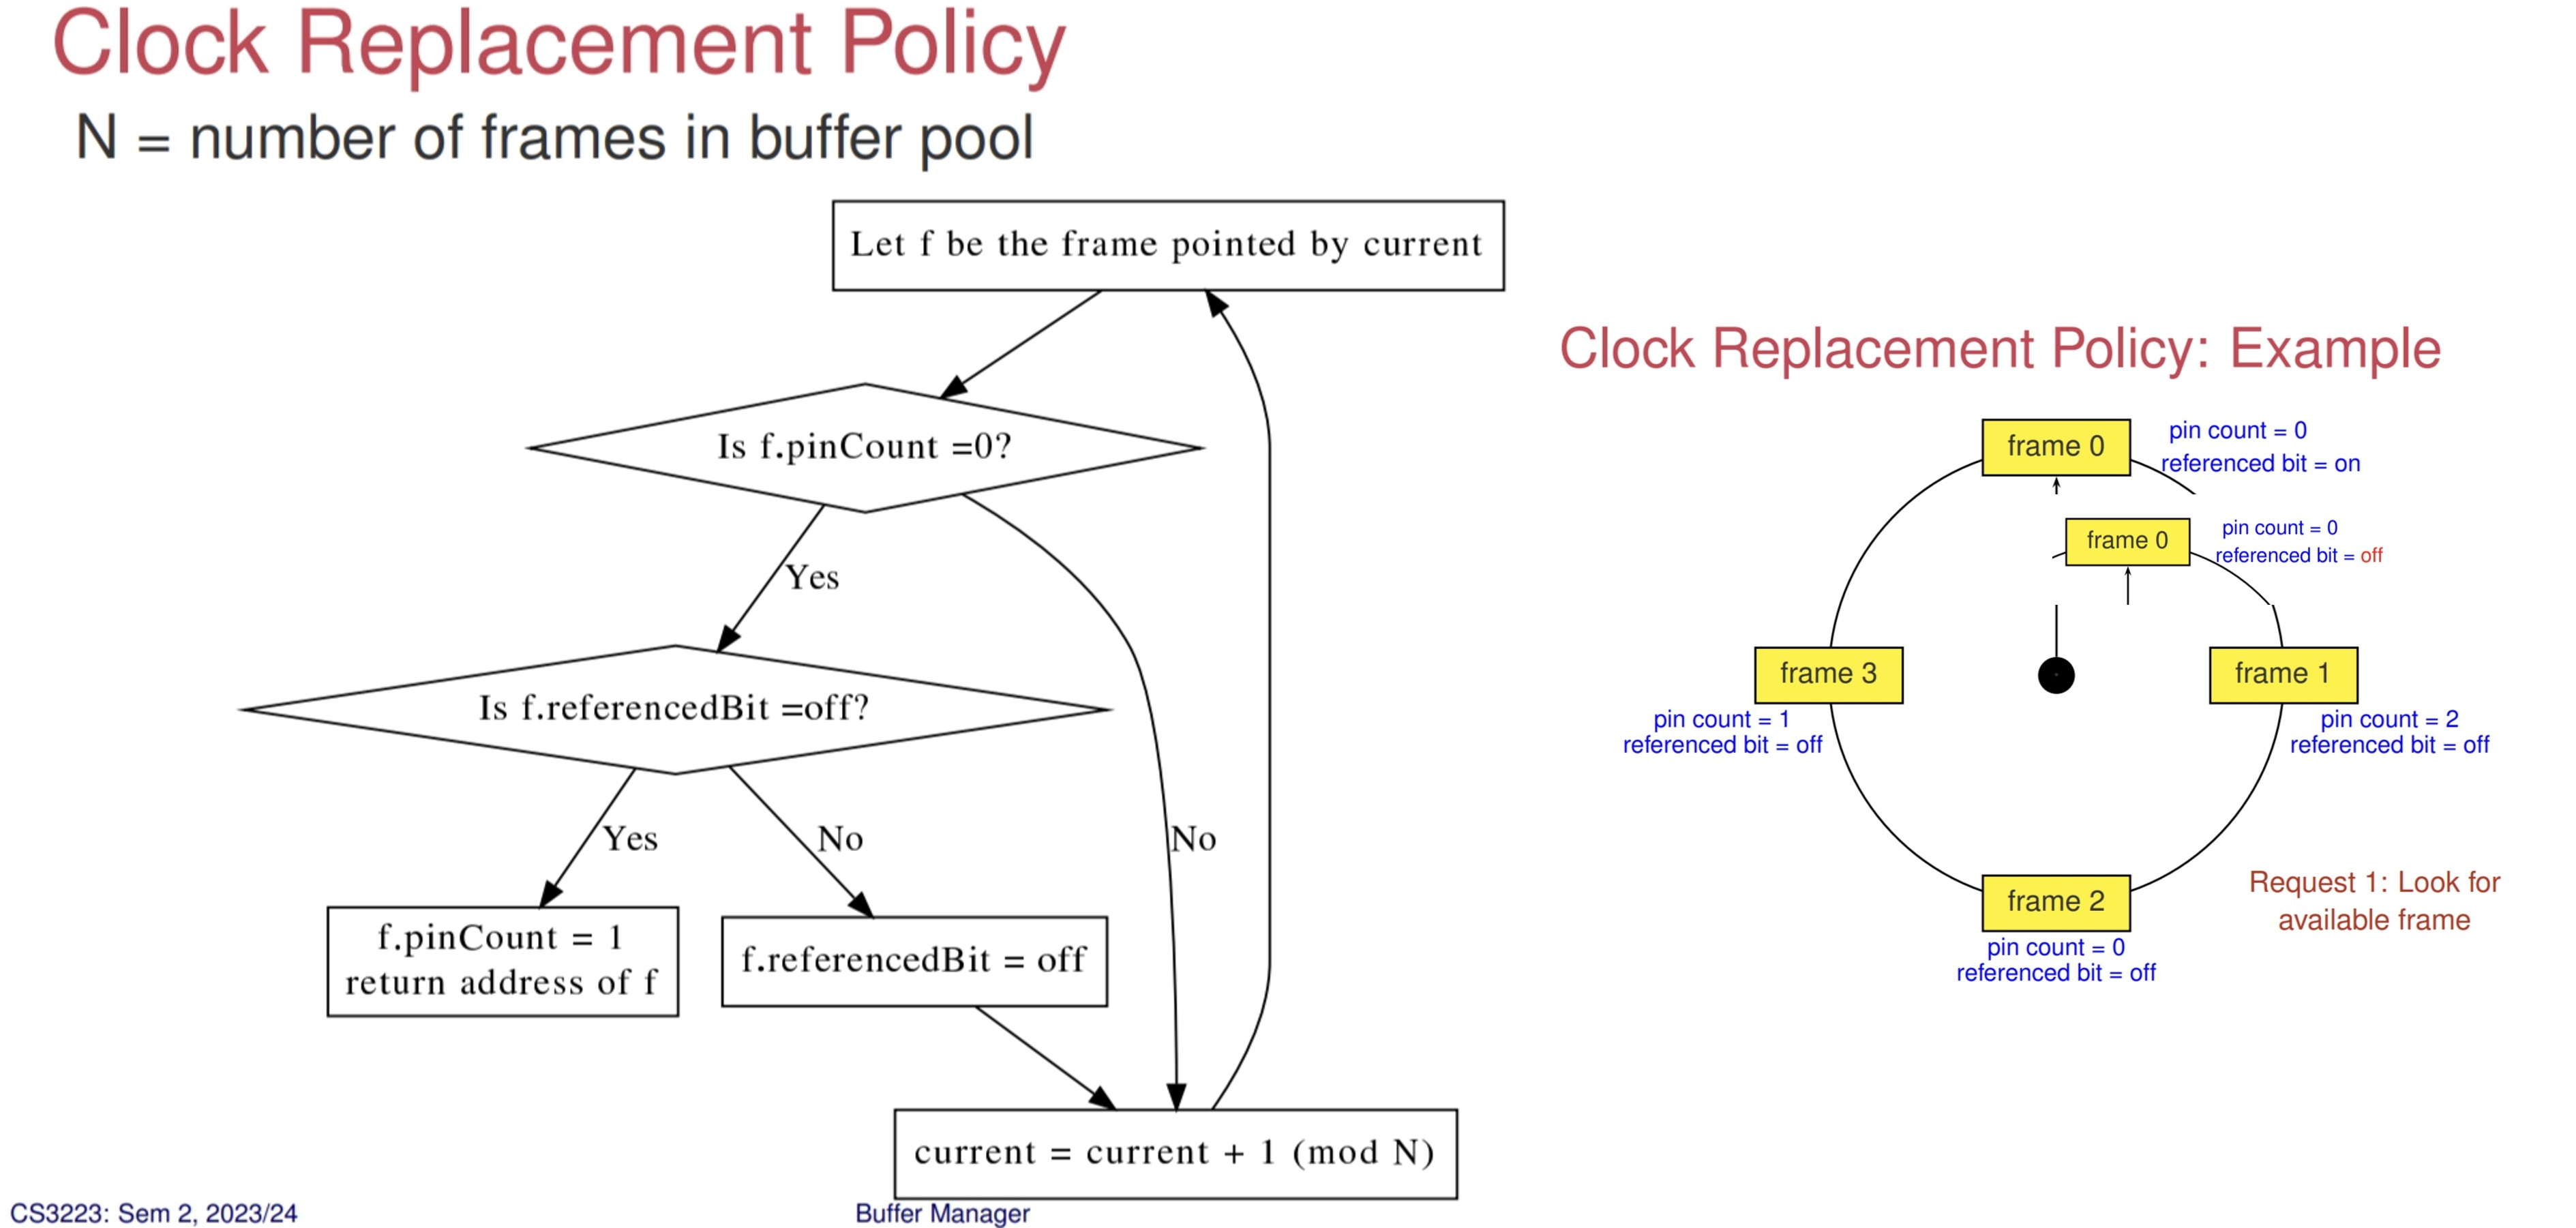
\includegraphics[width = 1\linewidth]{clockReplacementPolicy}}
\end{itemize}

\columnbreak

\subsection{Files}
\textbf{File Abstraction}
\begin{itemize}
	\item Each relation is a file of records.
	\item Each record has a unique record identifier called RID / TID.
	\item Common file operations: create/delete file, insert record, delete/get record with given RID, scan all records.
\end{itemize}
\textbf{File Organization}: Method of arranging data records in a file that is stored on disk.
\begin{itemize}
	\item \textbf{Heap file}: Unordered file
	\item \textbf{Sorted file}: Records order on some search key.
	\item \textbf{Hashed file}: Records located in blocks via a hash function.
\end{itemize}

\subsubsection{Heap File Implementations}
\centerline{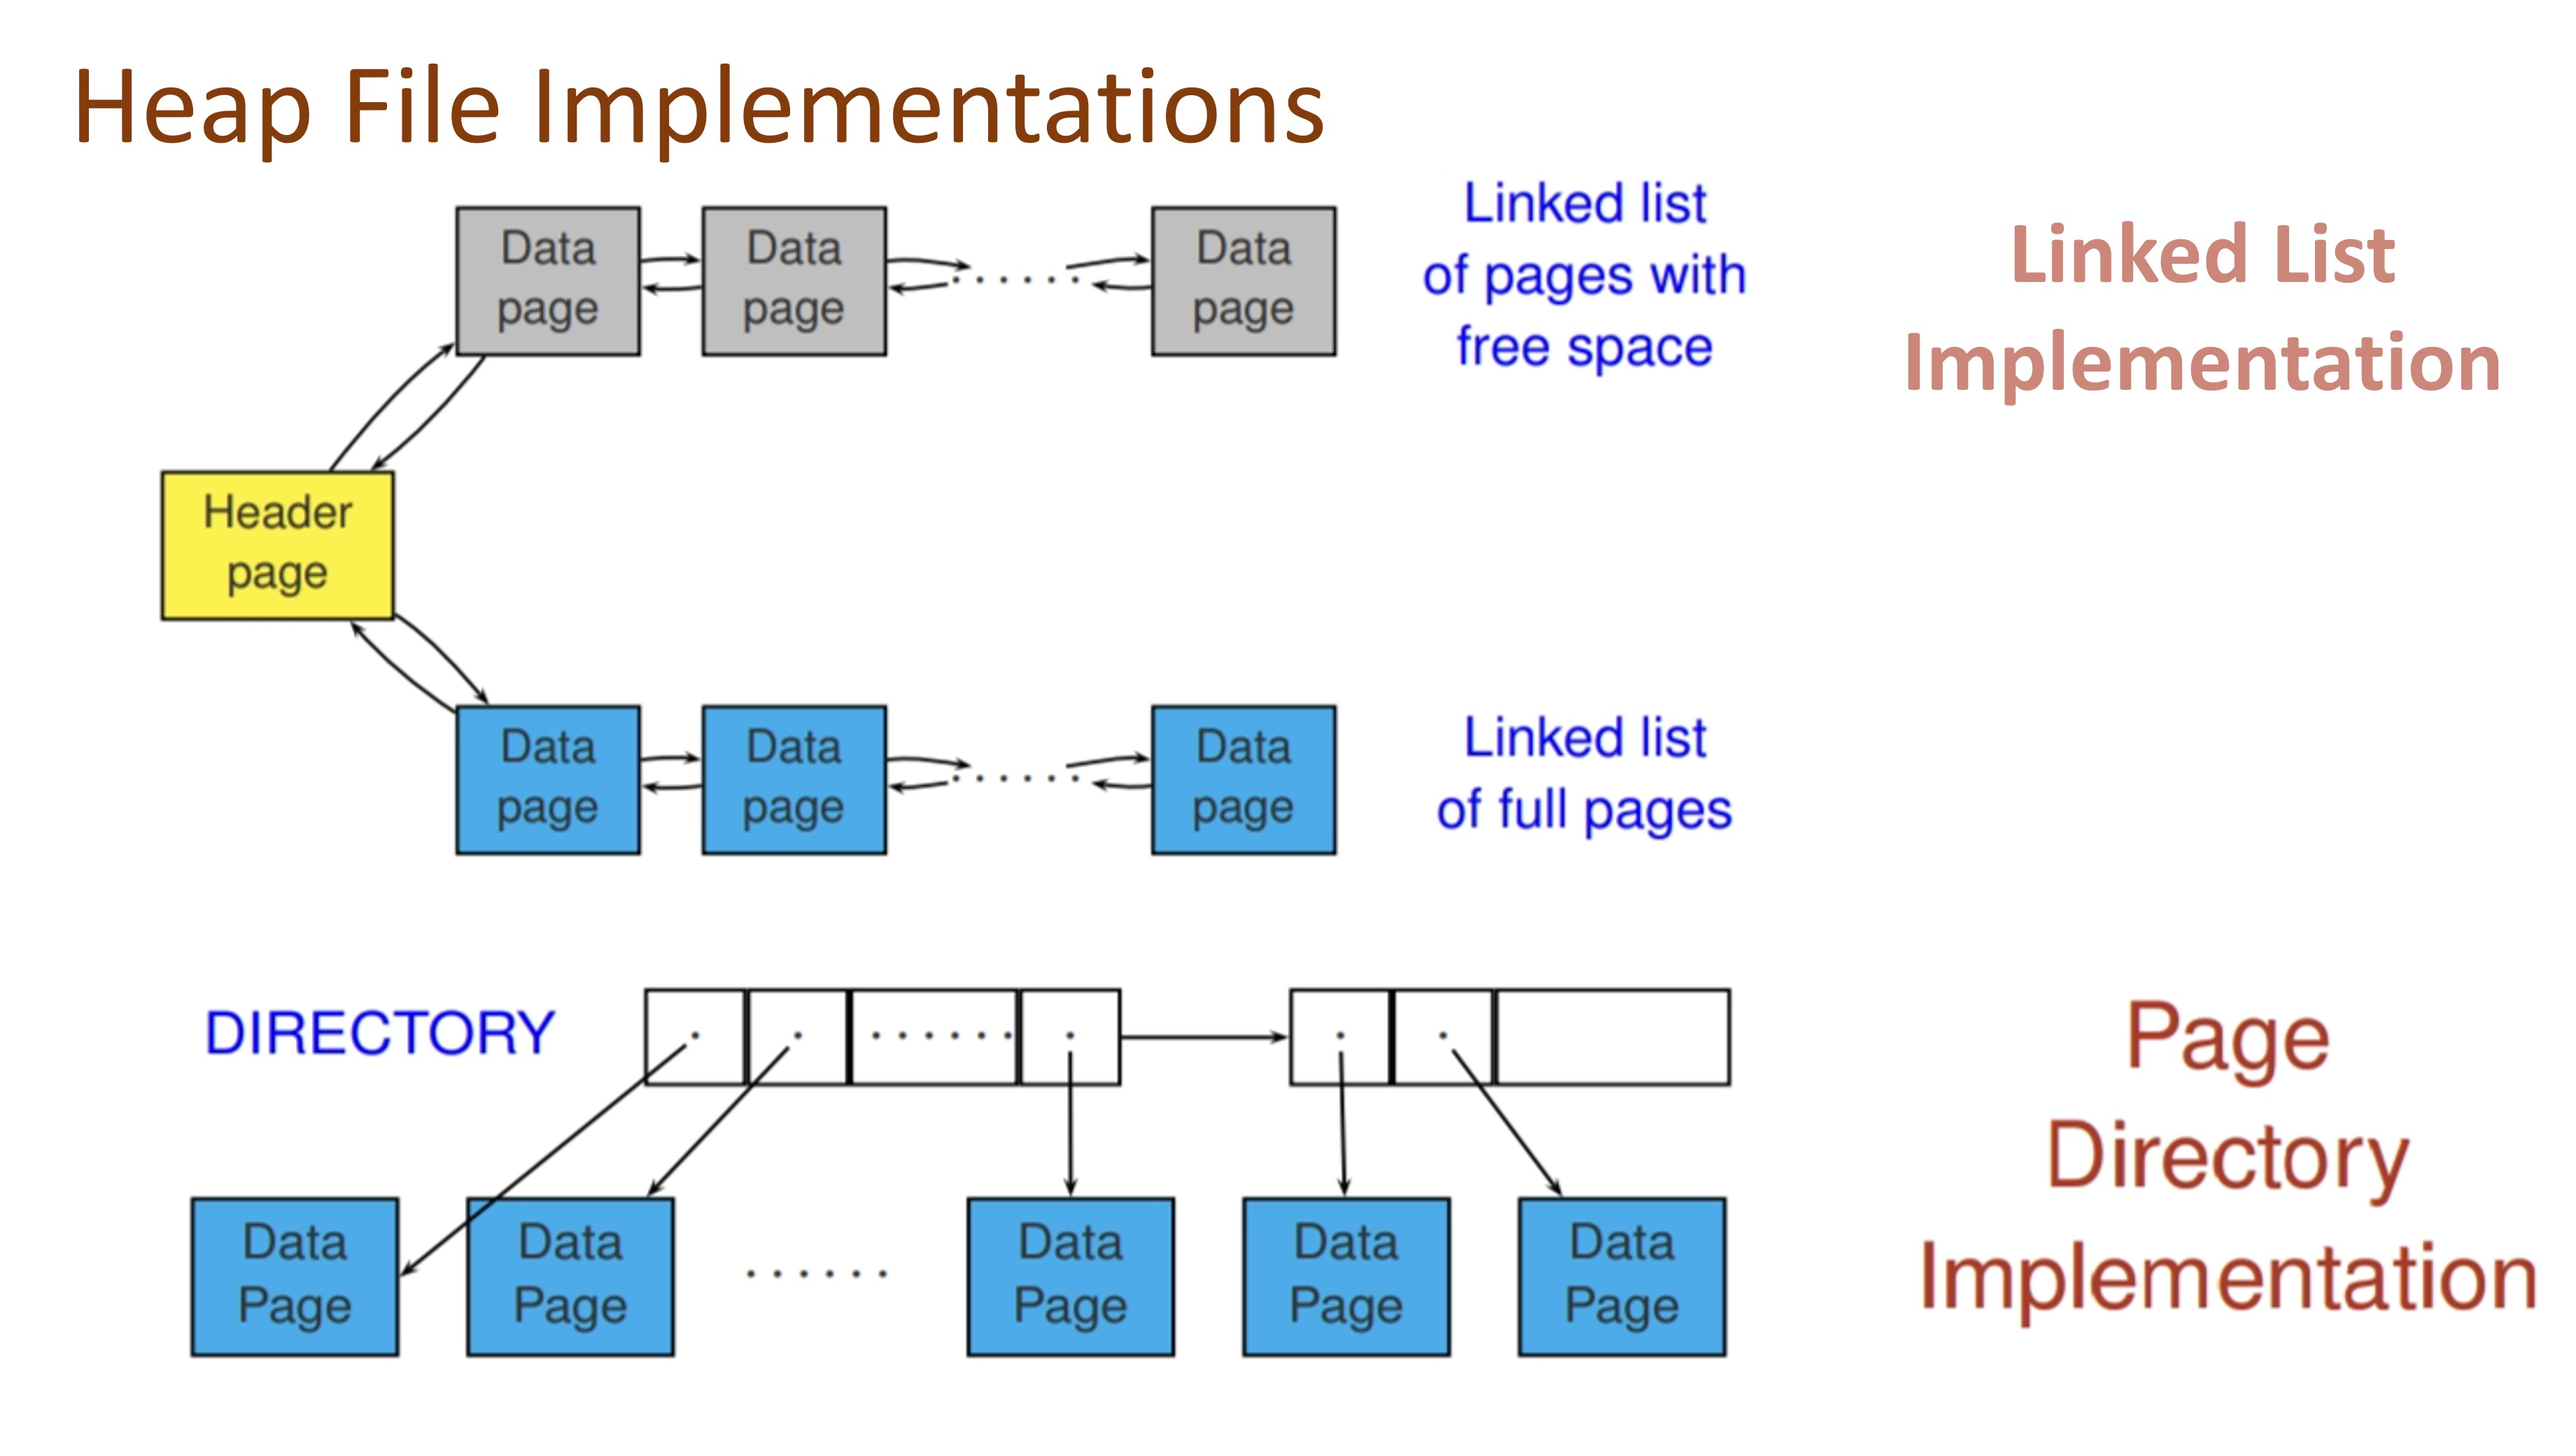
\includegraphics[width = 1\linewidth]{heapFileImplementations}}
\begin{itemize}
\item \textbf{Linked list implementation}: Two linked lists, one with pages with free space, other of completely full pages.
\item \textbf{Page Directory Implementation}: Two leveled implementation. Each big block is a disk block with some metadata. Each disk block has a number of data pages.
\end{itemize}

































\end{multicols*}
\end{document}
